\section{数式など}

{\TeX}では,数式を入力するときに数式モードに切り替える.
数式モードは,\verb|$a+b=c$|のようにドルマークで囲む,あるいは
\verb|\(a+b=\sqrt{c})\)|のように中カッコのコマンドでくくる方法がある.
式番号を伴う式などでは,\verb|\begin{equation}\end{equation}|で
囲む.詳しくはドキュメントを参照のこと.
以下は数式の表示例である.

文章中で書くと,\(a+b=\sqrt{c}\)のようになる.また数式番号を伴う独立した式では,
\begin{equation}
y_1(t) = A\cos(2\pi\omega t + \theta) + n_1(t)
\end{equation}
のようになる.

以下の例はソースを参照のこと.
\begin{equation}
\mathbfit{H}_n = \begin{bmatrix} x_1 & x_2\\ x_3 & x_4 \end{bmatrix}
\end{equation}

\begin{equation}
\mathrm{sinc\ }x = \frac{\sin x}{x}
\end{equation}


\section{ヒラギノ角ゴシックの全ウエイト使用例}

MacOS内蔵のヒラギノ角ゴシックには,W0$\sim$W9のウエイトがある.
内容が高度になるのでここでは説明しないが(このサンプルではPDFを読み込んでいます),
(u){p\LaTeX}では全てのウエイトを使用することが可能である.
そこで,最後にヒラギノ角ゴシックの各ウエイトとRobotoの各ウエイトを比べてみる.

\begin{figure}[ht]
\centering
\hspace*{-1em}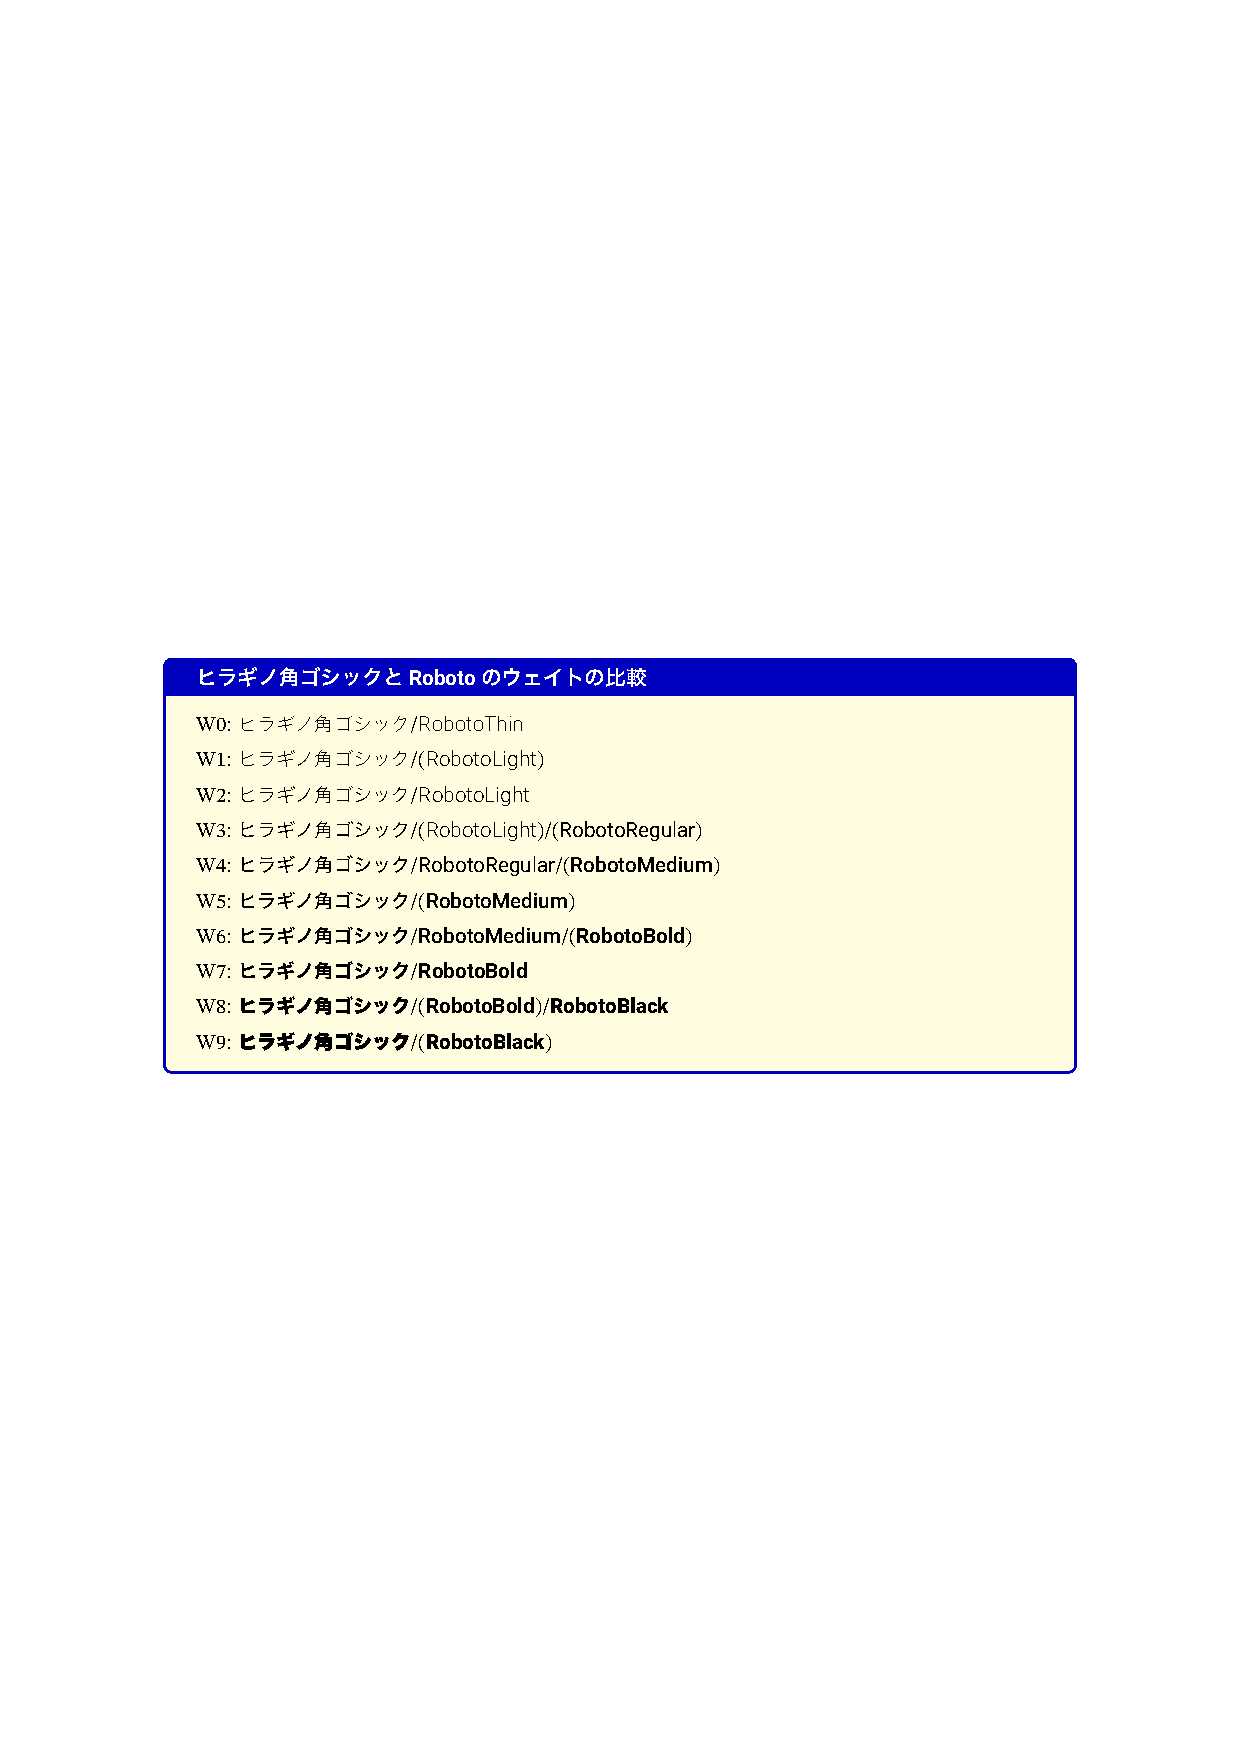
\includegraphics[scale=1.0,clip]{hira.pdf}
\label{hira}
\end{figure}
標準の設定では,通常フォントがヒラギノのW3とRobotoのレギュラー,太字では,ヒラギノのW6とRobotoのボールドが使用されるが,RobotoのレギュラーはヒラギノのW4とマッチし,ボールドはW7とマッチするように見える.
RobotoとSTIX Twoは同程度であるので,脚注\ref{太い}で,欧文フォントがヒラギノより若干太いのが気になると書いたが,実際そのとおりであることが確認できる.とはいえ,大きな差があるわけでもないので,気にしないならこのままでも問題ない.

